
\item A block of mass \(2 \, \text{kg}\) is free to move along the x-axis. It is at rest and from \( t = 0 \) onwards it is subjected to a time-dependent force \( F(t) \) in the x direction. The force \( F(t) \) varies with \( t \) as shown in the figure. The kinetic energy of the block after \( 4.5 \) seconds is
    \begin{center}
        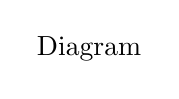
\begin{tikzpicture}
            % Placeholder for the actual diagram
            \node at (0,0) {Diagram};
        \end{tikzpicture}
    \end{center}
    \begin{tasks}(2)
        \task \(4.50 \, \text{J}\)
        \task \(7.50 \, \text{J}\)
        \task \(5.06 \, \text{J}\)\ans
        \task \(14.06 \, \text{J}\)
    \end{tasks}
